
% \definecolor{color1}{RGB}{145,30,180}
% \definecolor{color2}{RGB}{245,130,48}
% \definecolor{color3}{RGB}{230,25,75}
% \definecolor{color4}{RGB}{123,25,75}
% \definecolor{color5}{RGB}{44,160,44}

\definecolor{color1}{RGB}{116, 184, 22}
\definecolor{color2}{RGB}{77, 171, 247}
\definecolor{color3}{RGB}{99, 230, 190}
\definecolor{color4}{RGB}{132, 94, 247}
\definecolor{color5}{RGB}{250, 176, 5}

% 	\begin{wrapfigure}{r}{0.37\textwidth}
% \vspace{-15mm}
% 	% \begin{figure}[t] %插入图片
% 		\centering %图片居中
% 		\resizebox{.37\columnwidth}{!}{  %用于修改图片大小
			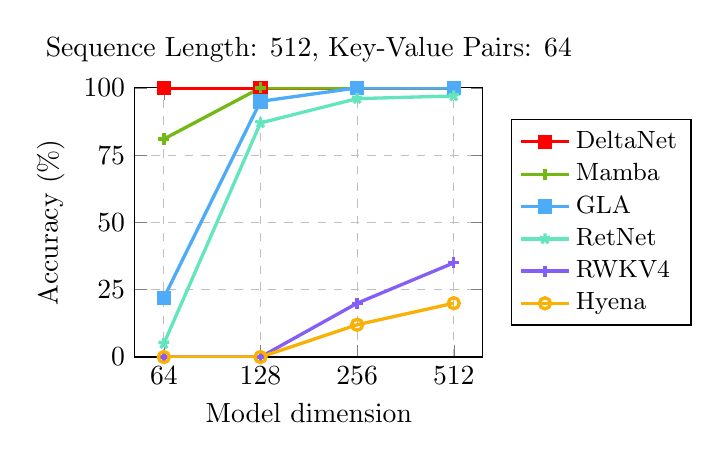
\begin{tikzpicture} %tikz图片
			\scalefont{1} %设置字体大小
% 			\begin{axis}[
%                 name=plot1,
% 			sharp plot, %控制线的风格
%         title style={align=right}, title={Sequence Length: 256\\Key-Value Pairs: 16},
%     % title={really\\ long title},%图像标题
% 			xmode=normal,% 控制坐标轴为线性
% %		ymode=log,% 控制坐标轴为对数
% 			xlabel=Model dimension, %x坐标名
% 			ylabel=Accuracy, %y坐标名
% 			width=6cm, height=5cm,  %设置长和宽
% 			% xmin=0,xmax=15,  % 设置x坐标范围
% 			ymin=0, ymax=100,  % 设置y坐标范围
% 			% xtick=, %指定x轴刻度值。如果为空，则自动设置刻度线。即分割坐标轴
%                 symbolic x coords={64,128,256,512},
% 			ytick={25,50,75,100}, %指定y轴刻度值。如果为空，则自动设置刻度线。即分割坐标轴
% 			xlabel near ticks, % 设置x坐标名位置靠近折线图
% 			ylabel near ticks, % 设置y坐标名位置靠近折线图
% 			ymajorgrids=true, % 启用/禁用 [公式] 轴上刻度线位置上的网格线
%                 xmajorgrids=true,
% 			grid style=dashed, % 设置网格线格式
% 			]
% 			%画第一条线，semithick设置线的粗细为0.6pt，mark是折线标示形状，options是mark形状的大小 ， olive!50!white是颜色，coordinates中包含要绘制的点的坐标
% 			\addplot+[very thick,mark=x,mark options={scale=0.5}, color=color1] plot coordinates { 
% 				(64,100)
% 				(128,100)
% 				(256,100)
% 				(512,100)
% 			};
			
% 			%画第二条线
% 			\addplot+[very thick, mark=square*, mark options={scale=1}, color=color2] plot coordinates {
% 				(64,99)
% 				(128,99)
% 				(256,99)
% 				(512,99)
% 			};
			
% 			%画第三条线
% 			\addplot+[very thick,mark=star,mark options={scale=1}, color=color3] plot coordinates {
% 				(64,97)
% 				(128,100)
% 				(256,100)
% 				(512,100)
% 			};
%    			\addplot+[very thick,mark=+,mark options={scale=1}, color=color4] plot coordinates {
% 				(64,0)
% 				(128,0)
% 				(256,70)
% 				(512,78)
% 			};

% 			\addplot+[very thick,mark=o,mark options={scale=1}, color=color5] plot coordinates {
% 				(64,0)
% 				(128,12)
% 				(256,50)
% 				(512,70)
% 			};

% 			\end{axis}
			\begin{axis}[
                name=plot2,
                % at={(plot1.south east) },
			sharp plot, %控制线的风格
        title style={align=right},
        title={Sequence Length: 512, Key-Value Pairs: 64},
			xmode=normal,% 控制坐标轴为线性
%		ymode=log,% 控制坐标轴为对数
			xlabel=Model dimension, %x坐标名
			% ylabel=y, %y坐标名
			width=6cm, height=5cm,  %设置长和宽
			% xmin=0,xmax=20,  % 设置x坐标范围
			ymin=0, ymax=100,  % 设置y坐标范围
                symbolic x coords={64,128,256,512},
   			ytick={0,25,50,75,100}, %指定x轴刻度值。如果为空，则自动设置刻度线。即分割坐标轴,
         yticklabels={0,25,50,75,100},
			% ytick, %指定y轴刻度值。如果为空，则自动设置刻度线。即分割坐标轴
			xlabel near ticks, % 设置x坐标名位置靠近折线图
			ylabel near ticks, % 设置y坐标名位置靠近折线图
   ylabel=Accuracy (\%),
			ymajorgrids=true, % 启用/禁用 [公式] 轴上刻度线位置上的网格线
			xmajorgrids=true, % 启用/禁用 [公式] 轴上刻度线位置上的网格线
			grid style=dashed, % 设置网格线格式
			legend style={at={(1.6,0.5)},anchor=east, legend cell align=left, font=\small}, 
			]

   		\addplot[very thick, mark=square*, mark options={scale=1}, color=red] plot coordinates {
				(64,100)
				(128,100)
				(256,100)
				(512,100)
			};
			\addlegendentry{DeltaNet} 


			\addplot[very thick,mark=+,mark options={scale=1}, color=color1] plot coordinates { 
				(64,81)
				(128,100)
				(256,100)
				(512,100)
			};
			\addlegendentry{Mamba} 
			
			\addplot[very thick, mark=square*, mark options={scale=1}, color=color2] plot coordinates {
				(64,22)
				(128,95)
				(256,100)
				(512,100)
			};
			\addlegendentry{GLA} 
			

			\addplot[very thick, mark=star, mark options={scale=1}, color=color3] plot coordinates {
				(64,5)
				(128,87)
				(256,96)
				(512,97)
			};
			\addlegendentry{RetNet}  

			\addplot[very thick, mark=+, mark options={scale=1}, color=color4] plot coordinates {
				(64,0)
				(128,0)
				(256,20)
				(512,35)
			};
			\addlegendentry{RWKV4}  

		\addplot[very thick, mark=o, mark options={scale=1}, color=color5] plot coordinates {
				(64,0)
				(128,0)
				(256,12)
				(512,20)
			};
			\addlegendentry{Hyena} 


			\end{axis}

			\end{tikzpicture}


 %  }
 %    \vspace{-6mm}
	% 	% \caption{The x-axis is the model dimension and the y-axis is accuracy on MQAR.} 
	% 	\caption{Accuracy (\%) on MQAR.} 
	% 	\label{fig:mqar} 
 %    \vspace{-7mm}

	% % \end{figure}/

	% \end{wrapfigure}